\section{Performance model}

\subsection{Performance model}
\begin{frame}
    \frametitle{Performance model}
	\begin{itemize}
		\item Two diffenent scenarios
		\begin{itemize}
			\item CPEs directly access global memory.(from global mem to register)  
			\item Three-level memory hierarchy.(REG-LDM-MEM)
		\end{itemize}
	\end{itemize} 
\end{frame}

\begin{frame}
	\frametitle{Performance model}
	\begin{figure}
		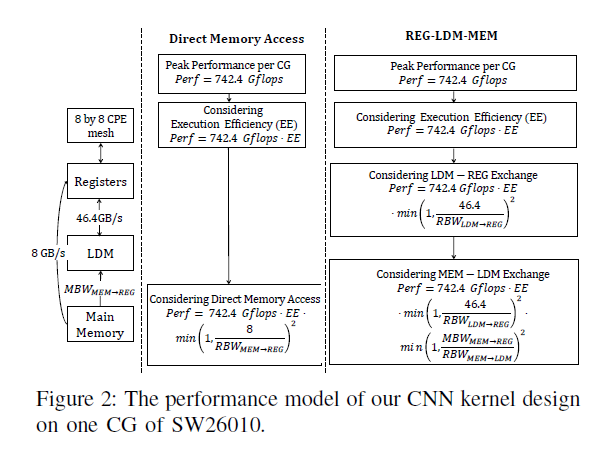
\includegraphics[scale=0.5]{figure/performancemodel.PNG}
	\end{figure}
\end{frame}

\begin{frame}
	\frametitle{$MBW_{MEM to LDM}$}
	\begin{figure}
		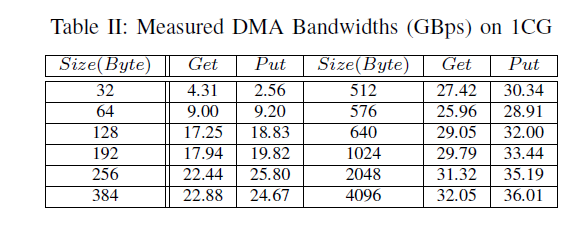
\includegraphics[scale=0.5]{figure/performancetable.PNG}
	\end{figure}
\end{frame}


	

